%
% k-gravitatzion.tex
%
% (c) 2017 Prof Dr Andreas Müller, Hochschule Rapperswil
%
\chapter{Gravitation%
\label{skript:kruemmusng:sectipn:gravitation}}
\lhead{Gravitation}
\rhead{}
Albert Einstein hat erkannt, dass die Wirkung der Gravitation 
durch die Krümmung des Raumes beschrieben werden muss.
\index{Einstein, Albert}
In den folgenden Abschnitten geben wir einen Ausblick darauf, wie
die moderne Physik unseren Raum als einen gekrümmten Raum beschreibt.
An einfachen Modellen soll gezeigt werden, wie man sich die Gravitationswirkung
als die Wirkung eines gekrümmten Raumes vorstellen kann, wie schwarze Löcher
beschrieben werden können, und wie alle diese Dinge tatsächlich gemessen
werden können.

\section{Äquivalenzprinzip}
\rhead{Äquivalenzprinzip}
Schon Galileo Galilei hat bemerkt, dass im Gravitationsfeld der Erde
jeder Körper unabhängig von seiner Masse die gleiche Beschleunigung $g$
erfährt.
Auch das Newtonsche Gravitationsgesetz beschreibt den Betrag der Kraft
zwischen zwei Massen $M$ und $m$ als
\[
F=\frac{KMm}{r^2}.
\]
Ein Teilchen der Masse $m$ wird daher nach dem zweiten Newtonschen Gesetz
$F=ma$ immer mit den Betrag
\[
\frac{KM}{r^2}
\]
haben.
Die Beschleunigung eines Teilchens ist daher unabhängig von der Masse.
Diese {\em Äquivalenz\-prinzip} genannte Beobachtung wurde von
Lor\'and Eötvös 1909 mit sehr grosser Genauigkeit nachgemessen und bestätigt.
In neuerer Zeit wurde die Genauigkeit nochmals um den Faktor $10^4$
verbessert.

Eine Folge des Äquivalenzprinzips ist auch, dass sich ein konstant
beschleunigtes Labor und ein Labor in einem homogenen Gravitationsfeld
nicht unterscheiden lassen (Abbildung~\ref{skript:gravitation:labor}).
\begin{figure}
\centering
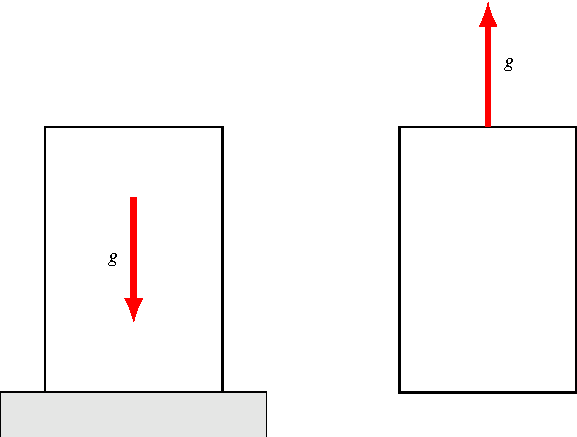
\includegraphics{chapters/tikz/labor.pdf}
\caption{Illustration des Äquivalenzprinzips.
Ein einem gleichmässig mit $g$ beschleunigten Labor (rechts)
misst man die gleiche Beschleunigung wie in einem homogenen
Gravitationsfeld (links).
\label{skript:gravitation:labor}}
\end{figure}
Ein beschleunigtes Koordinatensystem kann man zwar durch die
Koordinatentransformation
\begin{equation}
\left.
\begin{aligned}
t'&=t\\
x'&=x+\frac12gt^2
\end{aligned}
\right\}
\qquad
\Leftrightarrow
\qquad
\left\{
\begin{aligned}
t&=t'\\
x&=x'-\frac12gt'^2
\end{aligned}
\right.
\label{skript:gravitation:beschleunigt}
\end{equation}
erhalten, doch ist sie keine Lorentz-Transformation und erhält daher
die Minkowski-Metrik nicht.
Wenn es möglich sein soll, die Gravitationstheorie so zu verallgemeinern,
dass sie mit der speziellen Relativitätstheorie verträglich sein soll, dann
müssen wir auch andere Koordinatentransformationen als nur die
Lorenztransformation zulassen.
Das bedeutet aber, dass wir nicht mehr darauf beharren dürfen, dass
sich die Metrik in der Form
\begin{equation}
-c^2\,dt^2 + dx^2 + dy^2  + dz^2
\label{skript:gravitation:standardform}
\end{equation}
schreiben lässt.
Wir lassen daher in Zukunft beliebige Koordinatentransformationen zulassen
und daher auch Metriken $g_{\mu\nu}$, die von der
Standardform~\eqref{skript:gravitation:standardform} abweichen.

Wir wollen die Metrik berechnen, die im festen Koordinatensystem
anzuwenden ist. 
Dazu müssen wir die Transformation zuerst mit $x^0$ und $x'^0$ 
darzustellen:
\begin{equation}
\left.
\begin{aligned}
x'^0 &= x^0 \\
x'^1 &= x^1+\frac{1}{2c^2}(x^0)^2
\end{aligned}
\right\}
\qquad
\Leftrightarrow
\qquad
\left\{
\begin{aligned}
x^0 &= x'^0 \\
x^1 &= x'^1 - \frac{1}{2c^2}(x'^0)^2
\end{aligned}
\right.
\end{equation}
Für die Transformation der Metrik werden die partiellen Ableitungen
benötigt:
\begin{equation}
\begin{aligned}
\frac{\partial x^0}{\partial x'^0}&=1,
&
\frac{\partial x^0}{\partial x'^1}&=0,
&
\frac{\partial x^1}{\partial x'^0}&=-\frac{1}{c^2}x'^0,
&
\frac{\partial x^1}{\partial x'^1}&=1,
\\
\frac{\partial x'^0}{\partial x^0}&=1,
&
\frac{\partial x'^0}{\partial x^1}&=0,
&
\frac{\partial x'^1}{\partial x^0}&=\frac{1}{c^2}x^0,
&
\frac{\partial x'^1}{\partial x^1}&=1.
\end{aligned}
\end{equation}
Die zugehörige Transformationsmatrix ist also
\begin{equation}
\frac{\partial (x^0, x^1)}{\partial (x'^0, x'^1)}
=
\begin{pmatrix}
1&0\\
-\frac1{c^2}x'^0&1
\end{pmatrix},
\qquad
\frac{\partial (x'^0, x'^1)}{\partial (x^0, x^1)}
=
\begin{pmatrix}
1&0\\
\frac1{c^2}x^0&1
\end{pmatrix}.
\end{equation}
Im $(x^0,x^1)$-Koordinatensystem wird die Metrik durch die Matrix
\[
g_{\mu\nu}
=
\begin{pmatrix}-1&0\\0&1\end{pmatrix}
\]
ausgedrückt.
In $(x'^0,x'^1)$-Koordinaten muss die Matrix daher sein
\begin{align*}
g'_{\mu\nu}
&=
\begin{pmatrix}
1&0\\
\frac1{c^2}x'^0&1
\end{pmatrix}
\begin{pmatrix}
-1&0\\0&1
\end{pmatrix}
\begin{pmatrix}
1&\frac1{c^2}x'^0\\
0&1
\end{pmatrix}
=
\begin{pmatrix}
1&0\\
\frac1{c^2}x'^0&1
\end{pmatrix}
\begin{pmatrix}
-1&-\frac1{c^2}x'^0\\
 0& 1
\end{pmatrix}
\\
&=
\begin{pmatrix}
-1&-\frac1{c^2}x'^0\\
-\frac1{c^2}x'^0&1+\frac1{c^4}(x'^0)^2
\end{pmatrix}.
\end{align*}
Die Metrik $g'_{\mu\nu}$ ist offenbar wieder symmetrisch.
Wir könnten die Christoffelsymbole ausrechnen und die Geodäten
bestimmen, wir würden die Transformation von Geraden aus dem
$(x,t)$-Koordinatensystem finden.

\section{Newtonsche Gravitationstheorie%
\label{skript:section:newtonschegravitationstheorie}}
\rhead{Newtonsche Gravitationstheorie}
Als ersten Schritt in Richtung auf eine allgemeine Gravitationstheorie
zeigen wir, wie auch die Bahnen in einem Newtonschen Gravitationsfeld 
als Geodäten eines Zusammenhangs schreiben lassen.
Wer verwenden dazu aber nicht die Metrik und den daraus abgeleiteten 
Zusammenhang, dies hat erst die Einsteinsche Theorie geschafft.

\subsection{Schwerkraft}
Das Newtonsche Gravitationsgesetz beschreibt die Beschleunigung, die
auf ein Teilchen in einem Gravitationsfeld wirkt, welches von einer
Masse $m$ erzeugt wird.
Der Betrag der Kraft ist umgekehrt proportional zum Quadrat der
Entfernung.
Der Kraftvektor kann deshalb als
\begin{equation}
\vec F = -\frac{KM}{r^2}\cdot\frac{\vec r}{r}
\label{skript:gravitation:gkraft}
\end{equation}
geschrieben werden.
Die Bewegungsgleichung ist daher 
\begin{equation}
\ddot x^k = -\frac{KM}{r}\cdot\frac{x^k}{r},
\qquad\text{mit}\qquad r = \sqrt{(x^1)^2+(x^2)^2+(x^3)^2},
\label{skript:gravitation:bewegungsgleichung}
\end{equation}
es kommt nur die Beschleunigung und die Position vor.

In den Geodätengleichungen 
\[
\ddot x^\mu = -\Gamma^\mu_{\alpha\nu}\dot x^\alpha\dot x^\nu
\]
kommt dagegen auf der rechten Seite auch die Geschwindigkeit vor.
Es ist daher nicht unmittelbar klar, wie die Bewegungsgleichung als
Geodätengleichung geschrieben werden klar.

Wir beschreiben die Bewegung wieder in einem vierdimensionalen Raum,
also als Kurve
\[
t\mapsto (t,x^1(t),x^2(t),x^3(t)),
\]
also mit $x^0(t)=t$.
Für eine solche Parametrisierung gilt $\dot x^0(t)=1$.
In der Geodätengleichung können wir daher die Terme mit mit Index $0$
separat behandelt werden:
\[
\ddot x^\mu
=
-\Gamma^\mu_{00}
-\Gamma^\mu_{k0}\dot x^k -\Gamma^\mu_{0l}\dot x^l
- \Gamma^\mu_{kl}\dot x^k\dot x^l
\]
Da in der Bewegungsgleichung~\eqref{skript:gravitation:bewegungsgleichung}
auf der rechten Seite keine Geschwindigkeiten vorkommen, darf nur der
erste Term stehen bleiben, also
\begin{equation}
\Gamma^k_{00} = \frac{KM}{r^2}\cdot \frac{x^k}{r},\qquad k=1,\dots,3.
\label{skript:gravitation:newtonzusammenhang}
\end{equation}
Da die erste Komponente der Geodäte $x^0(t)=t$ ist und seine zweite
Ableitung $\ddot x^0(t)=0$, muss auch $\Gamma^0_{\alpha\nu}=0$ sein.
Die einzigen nicht verschwindenden Zusammenhangskoeffizienten sind
\eqref{skript:gravitation:newtonzusammenhang}.

Man kann für den Zusammenhang~\eqref{skript:gravitation:newtonzusammenhang}
auch die Definition des Riemann-Krümmungstensors anwenden.
Die Rechnung zeigt aber, dass zwar einzelne Komponenten des Riemann-Tensors
nicht verschwinden, der Ricci-Tensor und damit auch der Einstein-Tensor
verschwinden dagegen identisch.
Diese Beschreibung der Gravitation führt also nicht auf das Modell
eines gekrümmten Raumes.

\subsection{Gravitationspotential}
Die potentielle Energie, die zur
Gravitationskraft~\eqref{skript:gravitation:gkraft} gehört, kann
mit Hilfe eines Wegintegrals berechnet werden.
Dazu verwenden wir einen Weg vom Punkt $P_1$ mit Radius $r_1$
zum Punkt $P_2$ mit Radius $r_2$ führt.
Da die Kraft immer radial wirkt, ist entlang des Weges nur die radiale
Komponente des Tangentialvektors massgebend.
Der Unterschied in der poteniellen Energie ist
\[
\Delta E
=
\int_{P_1}^{P_2} \vec F\cdot d\vec s
=
\int_{r_1}^{r_2} -\frac{KM}{r^2}\,dr
=
\biggl[
\frac{KM}{r}
\biggr]_{r_1}^{r_2}
=
GM\biggl(\frac{1}{r_2}-\frac{1}{r_1}\biggr).
\]
Legt man den Nullpunkt der potentiellen Energie ins unendliche, dann ist
das Potential einer Punktmasse mit Masse $M$ ist also
\begin{equation}
\varphi = \frac{KM}{r}.
\label{skript:gravitation:potential}
\end{equation}

Aus dem Potential kann man die Kraft mit Hilfe des Gradienten
berechnen.
Zur Berechnung brauchen wir die Ableitung von $r$ nach den Koordinaten.
Die Ableitung nach $x$ ist
\[
r=\sqrt{x^2+y^2+z^2}
\qquad\Rightarrow\qquad
\frac{\partial r}{\partial x}
=
\frac{1}{2r} \frac{\partial (x^2+y^2+z^2)}{\partial x}
=
\frac{1}{2r} 2x=\frac{x}{r}.
\]
Damit können wir jetzt die Ableitung des Potentials berechnen:
\begin{align*}
\frac{\partial}{\partial x}\frac1{r}
&=
-\frac{1}{r^2} \frac{\partial r}{\partial x}
=
-\frac{1}{r^2} \frac{x}{r}.
\end{align*}
Der Gradient
\[
\operatorname{grad}\varphi
=
-\frac{KM}{r^2}\cdot\frac1r\begin{pmatrix}x\\y\\z\end{pmatrix}
=
-\frac{KM}{r^2}\cdot\frac{\vec r}{r} = \vec F
\]
stimmt mit der Gravitationskraft überein.

Für eine ausgedehnte Masseverteilung mit Dichte $\varrho$ kann man das
Potential als Überlagerung von einzelnen Potentialen der
Form~\eqref{skript:gravitation:potential} berechnen.
%Das Integral
%\[
%\varphi(\vec r)
%=
%G\int_{\mathbb R^3} \frac{\varrho(\vec r')}{|\vec r-\vec r'|}\,d^3r',
%\]
%wobei das Integral als Volumen-Integral über alle Vektoren $\vec r'$
%zu erstrecken ist.
Eine solche Beschreibung
ist allerdings für unsere Zwecke nicht sehr nützlich.

Eine besser geeignete Beschreibung können wir aus dem Gausschen
Divergenzsatz erhalten.
Eine zweidimensionale Version dieses Satzes können wir
aus dem Satz von Green~\eqref{skript:kruemmung:satz:green}
erhalten.
Dazu verwenden wir die Funktionen 
\[
f(x)=-\frac{\partial \varphi}{\partial x}
\qquad\text{und}\qquad
g(x)=\frac{\partial \varphi}{\partial y}.
\]
Die linke Seite des Satzes von Green ist das Integral
\begin{equation}
\oint_{C}
\frac{\partial \varphi}{\partial x} \dot (-x(s))
\frac{\partial \varphi}{\partial y} \dot y(s)
\,ds
\label{skript:gravitation:fluss1}
\end{equation}
Der Vektor
\[
\vec o(s) = \begin{pmatrix}-\dot x(s)\\\dot y(s)\end{pmatrix}
\]
steht senkrecht auf dem Rand des Gebietes.
Im Integral~\eqref{skript:gravitation:fluss1} wird das Skalarprodukt
diese Vektors mit dem der Gravitationskraft $\vec F$ verwendet,
man nennt
\[
\oint_{C} \vec F\cdot \vec o(s)\,ds
\]
den Fluss des Vektorfeldes durch die Kurve $C$.
Auf der rechten Seite findet man dann 
\[
\int \frac{\partial g}{\partial x}-\frac{\partial f}{\partial x}\,dx\,dy
=
\int
\frac{\partial^2\varphi}{\partial x^2}
+
\frac{\partial^2\varphi}{\partial y^2}
\,dx\,dy
=
\int\Delta\varphi \,dx\,dy.
\]
Der Satz von Gauss besagt daher
\[
\oint_{C} \vec F\cdot d\vec o
=
\int_{D} \Delta\varphi\,dx\,dy.
\]
In dieser zweidimensionalen Darstellung nützt uns der Satz allerdings
wenig, denn das Gravitationsfeld ist natürlich dreidimensional.
Die dreidimensionale Version kann jedoch mit ganz ähnlichen Ideen
bewiesen werden wie der Satz von Green:

\begin{satz}[Gauss] Ist $\vec v$ ein Vektorfeld in
einem dreidimensionalen Gebiet $D\subset R^3$ mit Randfläche $S=\partial D$,
dann gilt
\begin{equation}
\oint_S \vec v\cdot d\vec o
=
\int_D 
\frac{\partial v_x}{\partial x}
+
\frac{\partial v_y}{\partial y}
+
\frac{\partial v_z}{\partial z}
\,dx\,dy\,dz
=
\int_D \operatorname{div}\vec v\,dx\,dy\,dz.
\label{skript:gravitation:gausssatz}
\end{equation}
Darin ist $\vec o$ ein Vektor ein nach aussen zeigender Vektor, der
senkrecht auf der Oberfläche des Gebietes steht.
\end{satz}

Der Nutzen dieses Satzes ist, dass man den Fluss des Schwerkraftfeldes
$\vec F$ einer Punktladung durch eine mit der Masse konzentrischen
Kugel auch direkt berechnen kann.
Dann hat nämlich $\vec F$ auf der Kugeloberfläche $S^2$ überall den gleichen
Betrag, und die Richtung ist immer senkrecht auf der Kugeloberfläche.
Das Skalarprodukt in~\eqref{skript:gravitation:gausssatz} ist daher
einfach ein Produkt der Beträge und das Integral bekommt man durch
Multiplikation mit der Kugeloberfläche:
\[
\oint_{S^2_r} \vec F\cdot d\vec o
=
4\pi r^2
\frac{KM}{r^2}
=
4\pi KM.
\]
Der Fluss des Gravitationsfeldes mit Potential $\varphi$ durch einen
sehr kleinen Ball $B_r$ mit Radius $r$ hat daher den Wert
\[
\int_{S^2_r}\vec F\cdot d\vec o
=
4\pi K\int_{B_r} \varrho\,dx\,dy\,dz.
\]
Andererseits kann man nach dem Satz von Gauss auch die rechte 
Seite berechnen:
\begin{align*}
\int_{B_r} 4\pi G\varrho\,dx\,dy\,dz
&=
\int_{B_r}
\frac{\partial F_x}{\partial x}+
\frac{\partial F_y}{\partial y}+
\frac{\partial F_z}{\partial z}
\,dx\,dy\,dz
=
\int_{B_r}
\frac{\partial^2\varphi}{\partial x^2}+
\frac{\partial^2\varphi}{\partial y^2}+
\frac{\partial^2\varphi}{\partial z^2}
\,dx\,dy\,dz
\\
&=
\int_{B_r} \Delta\varphi\,dx\,dy\,dz.
\label{skript:gravitation:poisson-integral}
\end{align*}
mit der Abkürzung
\begin{equation*}
\Delta \varphi
=
\frac{\partial^2\varphi}{\partial x^2}+
\frac{\partial^2\varphi}{\partial y^2}+
\frac{\partial^2\varphi}{\partial z^2},
\end{equation*}
dem Laplace-Operator.
Da dies für Kugeln an beliebigen Punkten mit beliebigen Radien 
gilt, müssen die Integranden in~\eqref{skript:gravitation:poisson-integral}
übereinstimmen.
Es folgt, dass das Gravitationspotential $\varphi$ die Gleichung
\begin{equation}
\Delta \varphi = 4\pi G\varrho
\label{skript:gravitation:potentialgleichung}
\end{equation}
erfüllen.
Diese Gleichung werden wir später dazu verwenden, die Verbindung zwischen
der newtonschen und der einsteinschen Gravitationstheorie herzustellen.

\section{Schwache Felder und die Metrik}
Für schache Gravitationsfelder hat die Newtonsche Theorie gute Dienste
geleistet. 
Wir gehen daher davon aus, dass eine neue, allgemeinere Theorie die
newtonsche Theorie als Grenzfall erhalten muss.
Es muss also möglich sein, die Gravitationskräfte, die wir im 
Abschnitt~\ref{skript:section:newtonschegravitationstheorie} bereits
mit Hilfe des Zusammenhangs, also den Koeffizienten $\Gamma^\alpha_{\mu\nu}$
beschrieben haben, auch aus einer Metrik zu gewinnen.
Die Zusammenhangskoeffizienten in
Abschnitt~\ref{skript:section:newtonschegravitationstheorie} waren nicht
die Christoffelsymbole einer Metrik.

Wir möchten jetzt eine Metrik finden, die einerseits möglichst nahe
an der Minkovski-Metrik ist, deren zugehörige Geodäten andererseits die
Bewegung in einem schwachen Gravitationsfeld korrekt wiedergibt.
Als Metrik verwenden wir daher
\[
g_{\mu\nu}=\eta_{\mu\nu} + h_{\mu\nu}.
\]
Der erste Summan ist $\eta_{\mu\nu}$, der die Minkovski-Metrik 
wiedergibt, der zweite beschreibt die Abweichung,
wobei wir annehmen, dass $h_{\mu\nu}$ sehr klein ist.
Die zugehörigen Christoffelsymbole sind mit einiger, vorzugsweise
maschineller Rechnung zu finden.
Aus der Beschreibung des newtonschen Gravitationsgesetzes können wir
ablesen, dass wir die klassisch beobachteten Kräfte in Gestalt
des Christoffelsymbols
\[
\Gamma^{k}_{00}
=
-\frac{1}{2(h_{kk} + 1)}\frac{\partial h_{00}}{\partial x^k}
\]
wiederfinden müssen.
Da $h_{kk}$ im Vergleich zu $1$ sehr klein soll, bleibt
\[
\Gamma^{k}_{00}
=
-\frac{1}{2}\frac{\partial h_{00}}{\partial x^k}.
\]
Damit die Bahnen der newtonschen Gravitationstheorie entstehen, müssen
die $-\Gamma^k_{00}$ die Beschleunigungskomponenten des Gravitationsfelds
entstehen.
Diese bilden den Gradienten des Potentials des Gravitationsfeldes
\[
-\Gamma^k_{00} = -\frac{\partial\varphi}{\partial x^k}.
\]
Es folgt daher, dass $h_{00}=-2\varphi/c^2$ ist.
In erster Näherung beschreibt daher die Metrik
\begin{equation}
\begin{aligned}
g_{00} &= -1 -\frac{2\varphi}{c^2},
&&&
g_{kk} &= 1,\quad k=1,2,3.
\end{aligned}
\label{skript:gravitation:naeherung}
\end{equation}
Die gesuchte Theorie muss also in erster Näherung das newtonsche
Gravitationspotential in der $00$-Komponente des metrischen Tensors
verwenden.

\section{Einstein-Gleichungen für das Gravitationsfeld}
Die Näherung für schwache Felder dient uns nun als Leitfaden, um die
Einsteinschen Feldgleichungen herzleiten.
Einerseits beinhaltet die $g_{00}$-Komponente das Potential $\varphi$ des
Gravitationsfeldes, andererseits beschreibt die
Gleichung~\eqref{skript:gravitation:potentialgleichung}
den Zusammenhang zwischen dem Gravitationspotential und der
Masseverteilung.
Wir suchen jetzt eine Theorie, welche auch die übrigen Komponenten
des metrischen Tensors zu bestimmen erlaubt.
Wir gehen dazu mit Hilfe von Analogien vor, eine strenge Herleitung
der Gleichungen ist ebenfalls möglich, jedoch für dieses Skript etwas
zu aufwendig.

Für die folgenden mathematischen Objekte suchen wir einen Ersatz:
\begin{enumerate}
\item
Die Massedichte in 
Gleichung~\eqref{skript:gravitation:potentialgleichung}
muss durch eine Grösse ersetzt werden, die dem vorhandenen Vierer-Impuls
ebenfalls Rechnung trägt.
Ausserdem soll sie auch um andere Formen von Energie ergänzt werden 
können, um zum Beispiel die Gravitationswirkung der Energie eines
elektromagnetischen Feldes modellieren zu können.
\item
In Gleichung~\eqref{skript:gravitation:potentialgleichung}
kommen die zweiten Ableitungen nach den Koordinaten vor. 
Der Laplace-Operator lässt sich aber nur in der Minkowski-Metrik so 
formulieren, ausserdem trägt er der Zeitkoordinate nicht Rechnung.
Wir brauchen daher eine Grösse, die alle Koordinaten gleichwertig
behandelt, aber im Grenzfall schwacher Felder wieder auf den 
Laplace-Operator führt.
\item
Der Energieerhaltungssatz in Form der
Gleichung~\eqref{skript:speziell:energieerhaltung}
kann nicht aufrechterhalten werden, weil
Gravitationsfelder die Energie darin sich bewegender Massen verändern
können.
Es muss also eine Formulierung des Energie- und Impulserhaltungssatzes
gefunden werden, welche mit der erweiterten Theorie verträglich ist.
\end{enumerate}
Dieses Programm soll in den folgenden Abschnitten durchgeführt werden.
Am Ende soll in Analogie zur 
Potentialgleichung~\eqref{skript:gravitation:potentialgleichung}
eine Gleichung der Form
\[
\text{``Tensor zur Feldbeschreibung''}
=
4\pi K\cdot \text{``Tensor mit Energie und Impuls''}
\]
das Gravitationsfeld beschreiben.

\subsection{Massedichte und Energie-Impuls-Tensor}
Die Massedichte $\varrho$, die wir auf der rechten Seite der
Potentialgleichung~\eqref{skript:gravitation:potentialgleichung}
für das newtonsche Gravitationsfeld finden,
finden wir in der allgemeinen Theorie als $00$-Komponente
des Energie-Impuls-Tensors wieder.
Es ist daher naheliegend, dass auf der rechten Seite der gesuchten
Gleichung der Energie-Impuls-Tensor $T_{\mu\nu}$ stehen soll.

\subsection{Ricci- und Einstein-Tensor}
Auf der linken Seite der Gleichung erwarten wir ein Objekt, welches
sich aus den zweiten Ableitungen der $g_{\mu\nu}$ berechnen lässt.
Die Christoffel-Symbole enthalten die ersten Ableitungen von $g_{\mu\nu}$,
aber der Riemannsche Krümmungstensor enthält alle zweiten Ableitungen.
Wir müssen daher einen Tensor $G_{\mu\nu}$ konstruieren, der die Rolle
von $\Delta\varphi$ übernehmen kann.
In Analogie zur
Gleichung~\eqref{skript:gravitation:potentialgleichung}
erwarten wir dann eine Gleichung der Form
\[
G_{\mu\nu} = 4\pi KT_{\mu\nu}
\]
als allgemeine Feldgleichung für die Gravitation.

Der Riemann-Tensor $R^\mu\mathstrut_{\nu\varrho\sigma}$ hat zu viele
Indizes, es muss daraus erst ein Tensor zweiter Stufe hergestellt werden.
Dies ist zum Beispiel durch Verjüngung möglich.
Wegen der Symmetrieeigenschaften des Riemann-Tensors gibt es nicht allzuviele
Möglichkeiten, wie dies geschehen könnte.
Die Verjüngung 
\[
R_{\mu\nu} = R^{\alpha}\mathstrut_{\mu\alpha\nu}
\]
heisst der {\em Ricci-Tensor}.
Wegen
\[
R_{\mu\nu}
=
R^{\alpha}\mathstrut_{\mu\alpha\nu}
=
R^{\alpha}\mathstrut_{\nu\alpha\mu}
=
R_{\nu\mu}
\]
ist er symmetrisch.

% TODO: physikalische Interpretation

Diesen kann man weiter verjüngen und daraus den Krümmungs-Skalar
\[
R=R^\alpha\mathstrut_\alpha
\]
bilden.
Den gesuchten Tensor $G_{\mu\nu}$ können wir als Linearkombination
\[
G_{\mu\nu}=a R_{\mu\nu} + bg_{\mu\nu} R
\]
ansetzen.
Der Krümmungsskalar $R$ ist eine Invariante, wir brauchen den Faktor
$g_{\mu\nu}$, um daraus einen Tensor zu machen, der mit dem Ricci-Tensor
$R_{\mu\nu}$ linear kombiniert werden kann.
Die Koeffizienten $a$ und $b$ sind noch zu bestimmen.

\subsection{Energieerhaltung und Feldgleichungen}
Der Energie-Impuls-Tensor der speziellen Relativitätstheorie
% XXX Referenz
erfüllt den Erhaltungssatz
\[
\frac{\partial T^\mu_\nu}{\partial x^\mu}
=0.
\]
Wir können allerdings nicht annehmen, dass diese Formel weiterhin
gelten wird.
Das Gravitationsfeld kann ja zum Beispiel ein Gas beschleunigen und 
verdichten, so dass sich Energie- und Impuls-Inhalt verändern können.
Dies können durch die kovariante Ableitung
\[
0
=
\nabla_\mu T^\mu_\nu
=
\frac{\partial T^\mu_\nu}{\partial x^\mu}
-
\Gamma^{\mu}_{\alpha\mu}T^\alpha_\nu
\]
ausdrücken.
Die Terme mit den Christoffel-Symbolen zeigen, wie die Gravitationskraft
Energie und Impuls verändert.

Die zweite Bianchi-Identität
\begin{equation}
\nabla_\beta R^\alpha\mathstrut_{\mu\nu\sigma}
+
\nabla_\nu R^\alpha\mathstrut_{\mu\sigma\beta}
+
\nabla_\sigma R^\alpha\mathstrut_{\mu\beta\nu}
=0
\end{equation}
für den Riemannschen Krümmungstensor können wir nach den
Indizes $\alpha$ und $\nu$
\begin{equation}
\nabla_\beta R^\alpha\mathstrut_{\mu\alpha\sigma}
+
\nabla_\alpha R^\alpha\mathstrut_{\mu\sigma\beta}
+
\nabla_\sigma R^\alpha\mathstrut_{\mu\beta\alpha}
=0.
\end{equation}


